\documentclass[a4paper,11pt]{article}
\usepackage[margin=25mm,headheight=16pt,headsep=8pt]{geometry}
\usepackage[T1]{fontenc}
\usepackage[utf8]{inputenc}
\usepackage{lmodern}
\usepackage[english]{babel}
\usepackage{graphicx,booktabs,tabularx,array,enumitem,xcolor,tikz}
\usepackage{fancyhdr}
\usepackage[hidelinks]{hyperref}
\graphicspath{{figures/}}
\definecolor{reportblue}{HTML}{163A5F}
\definecolor{reportgray}{HTML}{5D6875}
\setlength{\parindent}{0pt}
\setlength{\parskip}{6pt}
\setlist{nosep,leftmargin=*}
\providecommand{\NoAutoSpacing}{}
\newcommand{\reportmeta}[2]{\textcolor{reportgray}{\scriptsize #1}\par\textbf{#2}\par}
\newcommand{\film}[1]{\mbox{\NoAutoSpacing #1}}
\newcommand{\varname}[1]{\texttt{#1}}
\addto\captionsenglish{\renewcommand{\contentsname}{Table of contents}}
\hypersetup{
  pdftitle={MCU --- Commercial and Critical Performance Analysis Report},
  pdfauthor={Lumu Bamana Manassé},
  pdflang={en}
}
\pagestyle{fancy}
\fancyhf{}
\fancyhead[R]{\color{reportgray}\small Lumu Bamana Manassé}
\fancyfoot[C]{\thepage}
\renewcommand{\headrulewidth}{0.4pt}
\renewcommand{\footrulewidth}{0pt}
\renewcommand{\headrule}{{\color{reportblue}\hrule width\headwidth height\headrulewidth}}

\begin{document}
\begin{titlepage}
  \begin{tikzpicture}[remember picture,overlay]
    \fill[reportblue] (current page.north west) rectangle
      ([yshift=-42mm]current page.north east);
    \fill[reportblue!15] ([yshift=-42mm]current page.north west) rectangle
      ([yshift=-47mm]current page.north east);
  \end{tikzpicture}
  \vspace*{18mm}
  {\color{white}\sffamily\Large DATA ANALYTICS PROJECT}\par
  \vspace{25mm}
  {\color{reportblue}\sffamily\fontsize{27}{32}\selectfont\bfseries
    MCU --- Commercial and Critical\\
    Performance Analysis Report\par}
  \vspace{5mm}
  {\large Analysis of Marvel Cinematic Universe Films --- Phases 1 to 5\par}
  \vspace{8mm}
  {\large Period analyzed: 2008--2024\par}
  \vspace{12mm}
  {\sffamily\large\bfseries\color{reportblue} Lumu Bamana Manassé --- Data Analyst\par}
  \vspace{2mm}
  {\sffamily\large MediJr\par}
  \vspace{2mm}
  {\sffamily\small\color{reportgray}%
    GitHub : MediJr ---
    \href{https://github.com/MediJr}{\textcolor{reportblue}{\nolinkurl{https://github.com/MediJr}}}\par}
  \vfill
  \begin{tabular}{@{}ll@{}}
    \reportmeta{Project}{Data Analytics} &
    \reportmeta{Period}{2008--2024}\\[7mm]
    \reportmeta{Scope}{Phases 1 to 5} &
    \reportmeta{Date}{September 2026}
  \end{tabular}
  \vfill
\end{titlepage}

\tableofcontents
\newpage

\section{Executive summary}

\subsection{Context}

The purpose of this analysis is to study the commercial and critical
performance of Marvel Cinematic Universe (MCU) films, in order to better
understand the trends observed within the catalogue and the factors
associated with film performance.

The analysis covers 34 films spanning MCU Phases 1 to 5, with information
on release dates, production budgets, box-office revenue, calculated
profit, return on investment (ROI), and critic and audience ratings.

\subsection{Key findings}

Across the dataset, the films represent a cumulative production budget of
6,947 million dollars and a cumulative worldwide box office of
31,129 million dollars.

The profit calculated according to the definition used in the dataset,
namely:
\begin{center}
\textbf{Profit = Worldwide box office $-$ Production budget}
\end{center}
amounts to 24,182 million dollars.

The catalogue's average IMDb rating is 7.26/10.

The phase-level analysis highlights substantial differences. Phase~3
shows the highest average box office, average profit, and overall ROI
in the dataset under study. Conversely, the average financial indicators
observed in Phase~5 are weaker than those of the earlier phases.

The analysis of relationships between variables also shows a positive
association between production budget and worldwide box office. A
positive association is also observed between IMDb rating and worldwide
box office.

These relationships must nevertheless be interpreted as statistical
associations and not as causal relationships.

\section{Objectives of the analysis}

The analysis addresses the following business brief:

\begin{quote}
``We want to analyze the commercial and critical performance of Marvel
Cinematic Universe films in order to better understand the factors
associated with a film's success.

In particular, we want to compare performance across MCU phases, examine
the relationship between investment and revenue, analyze film
profitability, and compare critical reception.

From this analysis, we want indicators and visualizations that will help
management better understand the catalogue's performance trends.''
\end{quote}

Based on this need, several analytical streams were selected:
\begin{itemize}
  \item measure commercial performance;
  \item compare the different MCU phases;
  \item analyze the relationship between investment and revenue;
  \item measure profitability;
  \item compare critical performance;
  \item identify factors associated with commercial performance;
  \item observe performance trends over time.
\end{itemize}

\section{Data and scope}

\subsection{Data source}

The dataset used contains 34 MCU films covering the period 2008--2024 and
includes 20 variables describing, in particular, temporal, commercial,
financial, and critical information about the films.

The main sources mentioned in the dataset documentation are:
\begin{itemize}
  \item IMDb;
  \item Box Office Mojo;
  \item Rotten Tomatoes;
  \item Wikipedia.
\end{itemize}

\subsection{Main variables}

The variables used in the analysis include, in particular:
\begin{itemize}
  \item film title;
  \item release date and year;
  \item MCU phase;
  \item chronological order;
  \item director;
  \item lead actor;
  \item runtime;
  \item production budget;
  \item worldwide box office;
  \item domestic box office;
  \item profit;
  \item ROI;
  \item domestic box-office share;
  \item IMDb rating;
  \item Rotten Tomatoes score;
  \item Metacritic score.
\end{itemize}

The dataset defines profit as the difference between worldwide box office
and production budget, while ROI corresponds to the return calculated
from profit and production budget.

\section{Data preparation and quality}

\subsection{Initial profiling}

A technical profiling of the dataset was carried out before the analysis.

The checks confirmed:
\begin{itemize}
  \item 34 rows and 20 columns;
  \item no missing values;
  \item no duplicates;
  \item 34 unique film identifiers;
  \item no inconsistency between phase and \varname{phase\_number};
  \item no inconsistency between \varname{release\_date} and
        \varname{release\_year};
  \item no critical values outside the expected ranges;
  \item no negative runtime.
\end{itemize}

\subsection{Consistency checks}

Additional checks were performed on the calculated variables.

The values of:
\begin{itemize}
  \item \varname{profit\_millions};
  \item \varname{domestic\_percentage};
  \item \varname{roi\_percentage}
\end{itemize}
were compared with their respective calculation formulas.

No inconsistency was detected.

\subsection{Cleaning}

The main correction identified concerned the data type of
\varname{release\_date}, which was initially stored as text.

The column was converted to a true date type before the cleaned dataset
was exported.

The cleaned file was then used for modeling and analysis in Power BI.

\textbf{Quality conclusion:} the checks performed indicate that the
dataset is consistent and suitable for the selected analysis, with a
data-type correction applied to the release date.

\section{Methodology and analytical architecture}

The analysis was carried out in several stages:

\begin{tabularx}{\linewidth}{@{}
  >{\centering\arraybackslash}p{14mm}
  >{\raggedright\arraybackslash}p{46mm}
  X
  @{}}
  \toprule
  \textbf{Step} & \textbf{Stage} & \textbf{Description} \\
  \midrule
  1 & Raw data & Starting point: MCU dataset \\
  2 & Profiling & Analysis of structure, types, missing values,
      duplicates, and distributions \\
  3 & Quality control & Verification of data validity, consistency,
      and integrity \\
  4 & Cleaning & Type correction and preparation of a usable file \\
  5 & Exploratory analysis & Data exploration with Python/Pandas
      and identification of the main findings \\
  6 & Modeling & Construction of the star schema in Power BI \\
  7 & Indicators & Creation of analytical measures with DAX \\
  8 & Visualization and analysis & Construction of the dashboard and
      interpretation of the results \\
  \bottomrule
\end{tabularx}

The Power BI model is based on a star schema comprising:
\begin{itemize}
  \item \varname{Fact\_Movie};
  \item \varname{Dim\_Movie};
  \item \varname{Dim\_Phase};
  \item \varname{Dim\_Date}.
\end{itemize}

The granularity of the fact table is:

\begin{center}
\textbf{1 film = 1 row in \varname{Fact\_Movie}.}
\end{center}

This structure makes it possible, in particular, to analyze performance
by film, phase, and release period.

\section{Results analysis}

\subsection{Catalogue overview}

The main catalogue indicators are as follows:

\begin{tabularx}{\linewidth}{@{}X r@{}}
  \toprule
  \textbf{Indicator} & \textbf{Result} \\
  \midrule
  Number of films & 34 \\
  Total budget & 6,947~M\$ \\
  Total worldwide box office & 31,129~M\$ \\
  Total calculated profit & 24,182~M\$ \\
  Average worldwide box office & 915.56~M\$ \\
  Average budget & 204.32~M\$ \\
  Average ROI per film & 339.58~\% \\
  Average IMDb rating & 7.26/10 \\
  Average Rotten Tomatoes score & 80.71~\% \\
  Average Metacritic score & 66/100 \\
  \bottomrule
\end{tabularx}

\begin{figure}[ht]
  \centering
  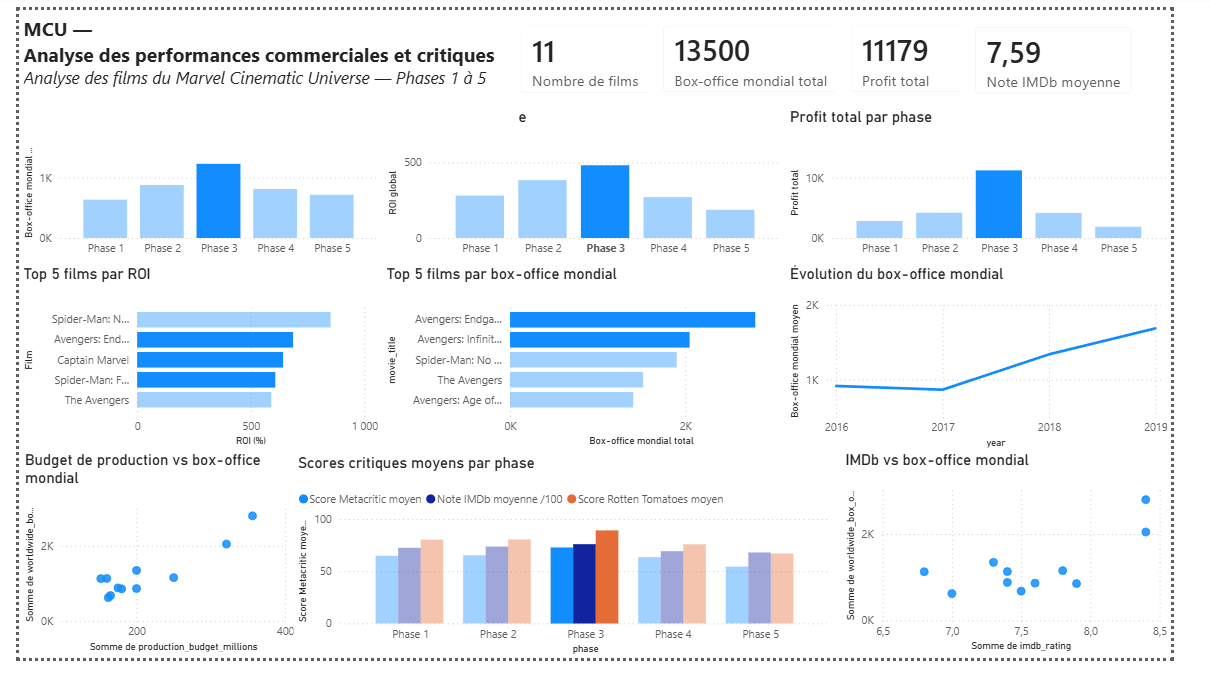
\includegraphics[width=\linewidth,keepaspectratio]{01_dashboard_global.png}
  \caption{Global MCU dashboard}
  \label{fig:dashboard-global}
\end{figure}

\subsection{Commercial performance by phase}

Average worldwide box office varies substantially across phases.

The observed averages are:

\begin{tabularx}{\linewidth}{@{}X r@{}}
  \toprule
  \textbf{Phase} & \textbf{Average worldwide box office} \\
  \midrule
  Phase 1 & 634.83~M\$ \\
  Phase 2 & 877.67~M\$ \\
  Phase 3 & 1,227.27~M\$ \\
  Phase 4 & 812.71~M\$ \\
  Phase 5 & 716.25~M\$ \\
  \bottomrule
\end{tabularx}

Phase~3 therefore shows the highest average worldwide box office within
the scope under study.

\begin{figure}[ht]
  \centering
  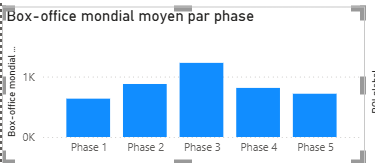
\includegraphics[width=\linewidth,keepaspectratio]{02_boxoffice_phase.png}
  \caption{Average worldwide box office by phase}
  \label{fig:boxoffice-phase}
\end{figure}

\subsection{Highest-grossing films}

The five films with the highest worldwide box office in the dataset are:

\begin{tabularx}{\linewidth}{@{}X r@{}}
  \toprule
  \textbf{Film} & \textbf{Worldwide box office} \\
  \midrule
  \film{Avengers: Endgame} & 2,798~M\$ \\
  \film{Avengers: Infinity War} & 2,048~M\$ \\
  \film{Spider-Man: No Way Home} & 1,902~M\$ \\
  The Avengers & 1,518~M\$ \\
  \film{Avengers: Age of Ultron} & 1,405~M\$ \\
  \bottomrule
\end{tabularx}

These results show that a small number of films contribute strongly to
the catalogue's overall commercial performance.

\begin{figure}[ht]
  \centering
  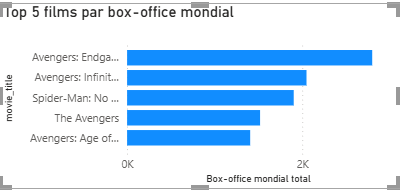
\includegraphics[width=\linewidth,keepaspectratio]{03_top5_boxoffice.png}
  \caption{Top 5 films by worldwide box office}
  \label{fig:top5-boxoffice}
\end{figure}

\subsection{Box-office trends over time}

The annual trend shows substantial variation in average commercial
performance over the period under study.

The highest levels are observed around 2018--2019, with a further
increase in 2024 in the dataset.

The trend is therefore not linear: several periods of growth and decline
are observed.

\begin{figure}[ht]
  \centering
  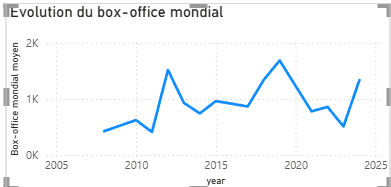
\includegraphics[width=\linewidth,keepaspectratio]{04_evolution_boxoffice.png}
  \caption{Worldwide box office over time}
  \label{fig:evolution-boxoffice}
\end{figure}

\subsection{Profitability and return on investment}

Overall ROI was calculated using the formula:
\begin{center}
\textbf{Overall ROI = Total profit / Total budget $\times$ 100}
\end{center}

This method measures the overall efficiency of investments rather than
simply averaging individual ROI values.

The results by phase are:

\begin{tabularx}{\linewidth}{@{}X r@{}}
  \toprule
  \textbf{Phase} & \textbf{Overall ROI} \\
  \midrule
  Phase 1 & 259.83~\% \\
  Phase 2 & 370.00~\% \\
  Phase 3 & 464.57~\% \\
  Phase 4 & 278.85~\% \\
  Phase 5 & 176.10~\% \\
  \bottomrule
\end{tabularx}

Phase~3 therefore has the highest overall ROI among the five phases
studied.

\begin{figure}[ht]
  \centering
  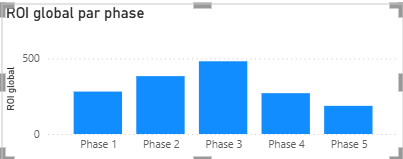
\includegraphics[width=\linewidth,keepaspectratio]{05_roi_phase.png}
  \caption{Overall ROI by phase}
  \label{fig:roi-phase}
\end{figure}

\subsection{Relationship between budget and box office}

The analysis of production budget and worldwide box office shows a
positive correlation of approximately 0.63 in the dataset.

This indicates that, within the data under study, films with higher
budgets also tend to be associated with higher box-office results.

However, this relationship does not establish that increasing the budget
automatically causes an increase in box office.

Other factors may be involved and are not directly measured in the
dataset.

\begin{figure}[ht]
  \centering
  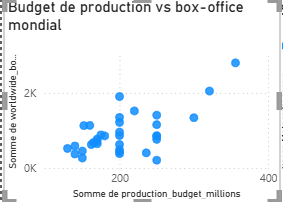
\includegraphics[width=\linewidth,keepaspectratio]{06_budget_boxoffice.png}
  \caption{Production budget vs worldwide box office}
  \label{fig:budget-boxoffice}
\end{figure}

\subsection{Films with the highest ROI}

The analysis of individual ROI identifies the films that generated the
highest return relative to their production budget.

The main results include, in particular:
\begin{itemize}
  \item \film{Spider-Man: No Way Home};
  \item \film{Avengers: Endgame};
  \item Captain Marvel;
  \item \film{Spider-Man: Far From Home};
  \item The Avengers.
\end{itemize}

ROI is used here as a complementary indicator to box office: a film
generating lower revenue may show a higher return if it was produced
with a relatively smaller investment.

\begin{figure}[ht]
  \centering
  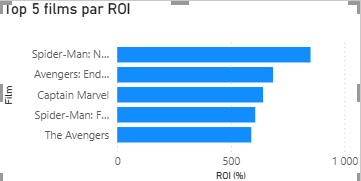
\includegraphics[width=\linewidth,keepaspectratio]{07_top5_roi.png}
  \caption{Top 5 films by ROI}
  \label{fig:top5-roi}
\end{figure}

\subsection{Profit by phase}

Total profit also varies substantially across phases.

The results show a particularly large contribution from Phase~3, which
generates the highest total profit in the dataset.

This observation is consistent with its high box-office level and
overall ROI.

\begin{figure}[ht]
  \centering
  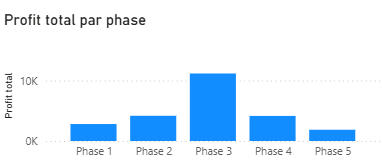
\includegraphics[width=\linewidth,keepaspectratio]{08_profit_phase.png}
  \caption{Total profit by phase}
  \label{fig:profit-phase}
\end{figure}

\subsection{Critical performance}

Three critical indicators were compared:
\begin{itemize}
  \item IMDb;
  \item Rotten Tomatoes;
  \item Metacritic.
\end{itemize}

To facilitate visual comparison, the IMDb rating was converted to a
100-point scale for this visualization only.

The observed averages by phase are:

\begin{tabularx}{\linewidth}{@{}X rrr@{}}
  \toprule
  \textbf{Phase} & \textbf{IMDb /100} & \textbf{Rotten Tomatoes} &
  \textbf{Metacritic} \\
  \midrule
  Phase 1 & 72.5 & 80.33 & 64.83 \\
  Phase 2 & 73.7 & 80.50 & 65.33 \\
  Phase 3 & 75.9 & 89.09 & 72.73 \\
  Phase 4 & 69.3 & 75.86 & 63.57 \\
  Phase 5 & 68.0 & 67.00 & 54.50 \\
  \bottomrule
\end{tabularx}

In the dataset under study, Phase~3 has the highest average critic
scores for all three indicators.

\begin{figure}[ht]
  \centering
  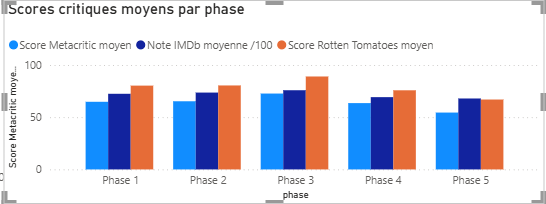
\includegraphics[width=\linewidth,keepaspectratio]{09_scores_critiques.png}
  \caption{Average critic scores by phase}
  \label{fig:scores-critiques}
\end{figure}

\subsection{Critical reception and box office}

The exploratory analysis shows a correlation of approximately 0.66
between IMDb rating and worldwide box office.

This relationship is stronger than those observed with Rotten Tomatoes
and Metacritic:
\begin{itemize}
  \item IMDb $\leftrightarrow$ Box office: 0.66
  \item Rotten Tomatoes $\leftrightarrow$ Box office: 0.44
  \item Metacritic $\leftrightarrow$ Box office: 0.42
\end{itemize}

In this dataset, IMDb rating therefore shows the strongest statistical
association with box office among the three critic indicators studied.

It is nevertheless important to recall that a correlation does not
demonstrate a causal relationship.

\begin{figure}[ht]
  \centering
  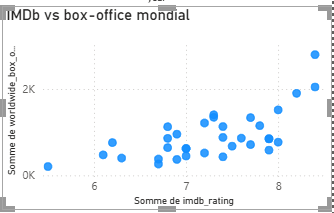
\includegraphics[width=\linewidth,keepaspectratio]{10_imdb_boxoffice.png}
  \caption{IMDb vs worldwide box office}
  \label{fig:imdb-boxoffice}
\end{figure}

\section{Conclusions}

The analysis of the 34 films under study highlights several findings.

\textbf{First,} commercial and financial performance varies substantially
across MCU phases. Phase~3 shows the highest average box-office levels
as well as the highest overall ROI and total profit within the scope
under study.

\textbf{Second,} a small number of films account for a large share of
the catalogue's commercial performance. \film{Avengers: Endgame},
\film{Avengers: Infinity War}, and \film{Spider-Man: No Way Home} are
among the films generating the highest worldwide box-office results.

\textbf{Third,} the analysis highlights a positive association between
production budget and worldwide box office. However, budget alone is
not sufficient to explain commercial performance.

\textbf{Fourth,} critical reception also shows a positive association
with box office, particularly in the case of IMDb rating. This
observation suggests that it may be relevant to study commercial and
critical indicators together.

\textbf{Finally,} the results show a decline in average indicators of
commercial performance, profitability, and critical reception between
some recent phases and Phase~3. This trend is a point of attention that
would warrant further analysis.

\section{Recommendations}

The following recommendations are based directly on the observed
results.

\subsection{Monitor commercial performance and profitability together}

Box office alone cannot measure the efficiency of an investment.

It is therefore recommended to track simultaneously:
\begin{itemize}
  \item budget;
  \item box office;
  \item profit;
  \item ROI.
\end{itemize}

This approach makes it possible to distinguish films that generate high
revenue from those that convert their investment into profit
efficiently.

\subsection{Compare performance across phases systematically}

The gaps observed between phases show the value of periodic monitoring
of indicators by period.

A dashboard comparing each new phase with previous phases could help
identify performance changes quickly.

\subsection{Examine factors associated with commercial performance}

The observed relationship between budget and box office, as well as
that between IMDb and box office, justifies further analysis of the
factors associated with commercial success.

A future analysis could include additional variables such as:
\begin{itemize}
  \item genre;
  \item lead character;
  \item director;
  \item franchise;
  \item release calendar;
  \item marketing;
  \item competition at the time of release;
  \item economic context;
  \item theatrical run length.
\end{itemize}

This would make it possible to go beyond the variables currently
available.

\subsection{Pay particular attention to the performance of recent
phases}

The average indicators observed for Phases 4 and 5 are lower than those
of Phase~3 on several dimensions.

It would therefore be relevant to carry out a more detailed analysis of
the films concerned in order to identify characteristics common to the
weakest and strongest performances.

This analysis should distinguish general trends from individual cases,
in order to avoid drawing conclusions from a limited number of films.

\subsection{Establish regular indicator monitoring}

The Power BI dashboard can serve as the basis for a performance
monitoring system.

The main indicators to track would include:

\textbf{Commercial performance}
\begin{itemize}
  \item worldwide box office;
  \item average box office;
  \item trend over time.
\end{itemize}

\textbf{Profitability}
\begin{itemize}
  \item profit;
  \item ROI;
  \item budget.
\end{itemize}

\textbf{Critical performance}
\begin{itemize}
  \item IMDb;
  \item Rotten Tomatoes;
  \item Metacritic.
\end{itemize}

Regular use of these indicators would make it possible to track the
catalogue's evolution and compare new releases with historical
performance.

\section{Limitations of the analysis}

Several limitations must be taken into account when interpreting the
results.

\subsection{Dataset size}

The analysis covers only 34 films. The results must therefore be
interpreted within the scope of this dataset and should not be
automatically generalized to the film industry as a whole.

\subsection{Definition of profit}

The profit used in this analysis corresponds to:
\begin{center}
\textbf{Worldwide box office $-$ production budget}
\end{center}

It is therefore a calculated indicator, and not necessarily a studio's
actual accounting profit.

Marketing, distribution, taxes, commissions, and other expenses are
not included in this formula.

\subsection{Correlation and causality}

The observed correlations make it possible to identify associations
between variables, but they do not establish causality.

For example, a positive correlation between budget and box office does
not necessarily mean that a higher budget directly generates higher
revenue.

\subsection{Unavailable variables}

Some factors that may influence commercial performance are not included
in the dataset.

The results should therefore be regarded as a descriptive and
exploratory analysis of the catalogue under study.

\section{Reporting tool}

An interactive Power BI dashboard was developed to support exploration
of the results.

The dashboard brings together:
\begin{itemize}
  \item the main KPIs;
  \item performance by phase;
  \item the highest-performing films;
  \item the trend over time;
  \item ROI;
  \item profit;
  \item critic scores;
  \item the budget/box-office relationship;
  \item the IMDb/box-office relationship.
\end{itemize}

The visualizations were selected on the basis of the business needs, in
order to avoid multiplying charts without additional analytical value.
The final selection includes 9 main visualizations covering the
commercial, financial, critical, and temporal dimensions of the
problem.

\begin{figure}[ht]
  \centering
  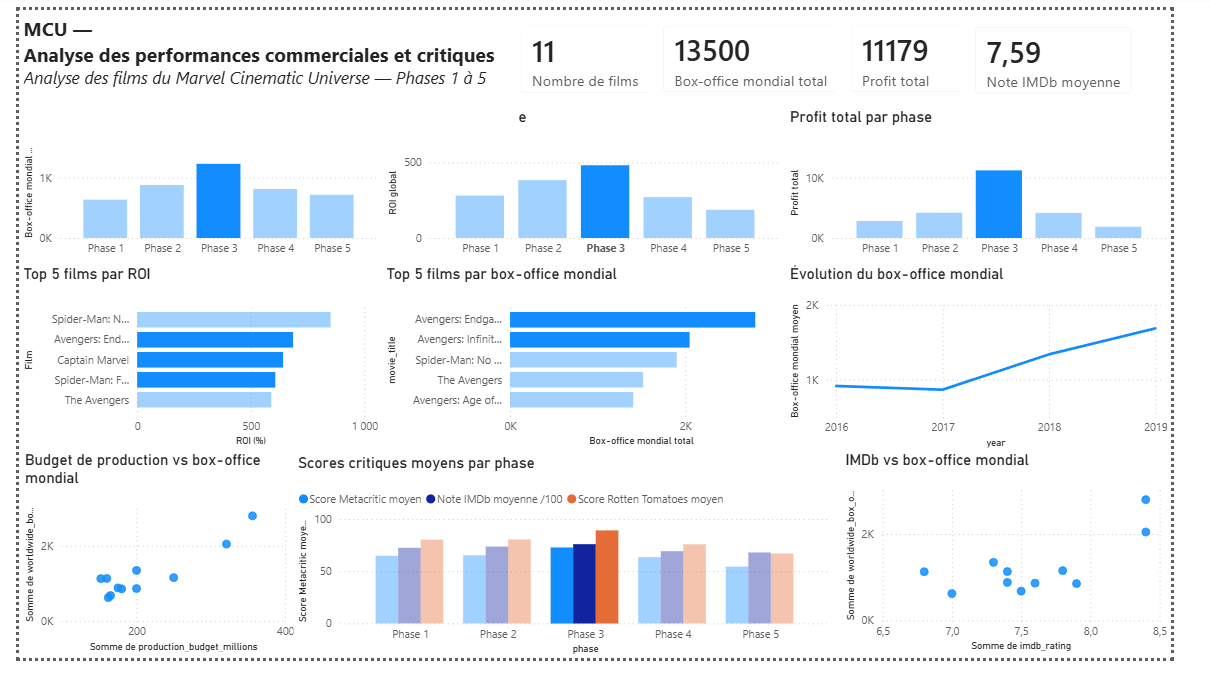
\includegraphics[width=\linewidth,keepaspectratio]{01_dashboard_global.png}
  \caption{Final Power BI dashboard}
  \label{fig:dashboard-final}
\end{figure}

\section{Final conclusion}

This analysis made it possible to build a complete chain from
understanding the business need through to interactive reporting of the
results.

The project covered:
\begin{itemize}
  \item problem framing;
  \item data inventory and understanding;
  \item profiling;
  \item quality control;
  \item cleaning;
  \item exploratory analysis with Python;
  \item dimensional modeling;
  \item creation of DAX measures;
  \item design of visualizations aligned with the business questions;
  \item delivery of an interactive Power BI dashboard.
\end{itemize}

The results provide a clearer understanding of performance differences
across MCU phases, the relationship between investment and revenue,
film profitability, and the associations between critical reception and
commercial performance.

The dashboard is therefore a synthesis tool for exploring catalogue
performance, while this report provides the context, methods, main
findings, conclusions, and avenues for further analysis.

\section{Appendices}

\subsection{Appendix A --- List of visualizations}

\begin{tabularx}{\linewidth}{@{}c X@{}}
  \toprule
  \textbf{No.} & \textbf{Visualization} \\
  \midrule
  1 & Average worldwide box office by phase \\
  2 & Top 5 films by worldwide box office \\
  3 & Worldwide box office over time \\
  4 & Overall ROI by phase \\
  5 & Production budget vs worldwide box office \\
  6 & Top 5 films by ROI \\
  7 & Total profit by phase \\
  8 & Average critic scores by phase \\
  9 & IMDb vs worldwide box office \\
  \bottomrule
\end{tabularx}

This selection corresponds to the final design defined for the
dashboard.

\subsection{Appendix B --- Project files}

The main technical files of the project include, in particular:
\begin{itemize}
  \item original dataset;
  \item cleaned dataset;
  \item Python scripts for profiling, cleaning, and analysis;
  \item Power BI model;
  \item analysis report.
\end{itemize}

\end{document}
